\documentclass{standalone}\usepackage[]{graphicx}\usepackage[]{color}
%% maxwidth is the original width if it is less than linewidth
%% otherwise use linewidth (to make sure the graphics do not exceed the margin)
\makeatletter
\def\maxwidth{ %
  \ifdim\Gin@nat@width>\linewidth
    \linewidth
  \else
    \Gin@nat@width
  \fi
}
\makeatother

\definecolor{fgcolor}{rgb}{0.345, 0.345, 0.345}
\newcommand{\hlnum}[1]{\textcolor[rgb]{0.686,0.059,0.569}{#1}}%
\newcommand{\hlstr}[1]{\textcolor[rgb]{0.192,0.494,0.8}{#1}}%
\newcommand{\hlcom}[1]{\textcolor[rgb]{0.678,0.584,0.686}{\textit{#1}}}%
\newcommand{\hlopt}[1]{\textcolor[rgb]{0,0,0}{#1}}%
\newcommand{\hlstd}[1]{\textcolor[rgb]{0.345,0.345,0.345}{#1}}%
\newcommand{\hlkwa}[1]{\textcolor[rgb]{0.161,0.373,0.58}{\textbf{#1}}}%
\newcommand{\hlkwb}[1]{\textcolor[rgb]{0.69,0.353,0.396}{#1}}%
\newcommand{\hlkwc}[1]{\textcolor[rgb]{0.333,0.667,0.333}{#1}}%
\newcommand{\hlkwd}[1]{\textcolor[rgb]{0.737,0.353,0.396}{\textbf{#1}}}%

\usepackage{framed}
\makeatletter
\newenvironment{kframe}{%
 \def\at@end@of@kframe{}%
 \ifinner\ifhmode%
  \def\at@end@of@kframe{\end{minipage}}%
  \begin{minipage}{\columnwidth}%
 \fi\fi%
 \def\FrameCommand##1{\hskip\@totalleftmargin \hskip-\fboxsep
 \colorbox{shadecolor}{##1}\hskip-\fboxsep
     % There is no \\@totalrightmargin, so:
     \hskip-\linewidth \hskip-\@totalleftmargin \hskip\columnwidth}%
 \MakeFramed {\advance\hsize-\width
   \@totalleftmargin\z@ \linewidth\hsize
   \@setminipage}}%
 {\par\unskip\endMakeFramed%
 \at@end@of@kframe}
\makeatother

\definecolor{shadecolor}{rgb}{.97, .97, .97}
\definecolor{messagecolor}{rgb}{0, 0, 0}
\definecolor{warningcolor}{rgb}{1, 0, 1}
\definecolor{errorcolor}{rgb}{1, 0, 0}
\newenvironment{knitrout}{}{} % an empty environment to be redefined in TeX

\usepackage{alltt}
\usepackage{tikz}
\usepackage{pgfplots}
\usepackage{fontspec}
\usetikzlibrary{decorations.text,pgfplots.groupplots,intersections,shapes.multipart}
\pgfplotsset{compat=1.7}

\definecolor{nice_blue}{HTML}{377EB8}
\definecolor{nice_green}{HTML}{4DAF4A}
\definecolor{nice_purple}{HTML}{984EA3}
\definecolor{nice_red}{HTML}{E41A1C}
\definecolor{nice_orange}{HTML}{FF7F00}

\pgfplotsset{
    simple graphs/.style={
        domain=0:12
        ,xmin=0
        ,xmax=12
        ,ymin=0
        ,ymax=12
        ,axis lines*=left
        ,xtick=\empty
        ,ytick=\empty
        ,every axis y label/.style={
            at={(axis description cs:0.09,.5)}
            ,rotate=90
            ,anchor=south},
        }
        ,every axis x label/.style={
            at={(axis description cs:0.5,-0.1)}
            ,anchor=south}
        }
        
% \makeatletter
% \tikzset{arc style/.initial={}}
% \pgfdeclareshape{three part circle}{
%     %\nodeparts{text,br,bl}
%     
%     \inheritsavedanchors[from=circle]
%     \inheritanchorborder[from=circle]
% 
%     \inheritanchor[from=circle]{center}
%     \inheritanchor[from=circle]{south}
%     \inheritanchor[from=circle]{west}
%     \inheritanchor[from=circle]{north}
%     \inheritanchor[from=circle]{east}
%     % etc.
% 
%     \inheritbackgroundpath[from=circle]
%     
% 
% 
%     \beforebackgroundpath{
%         % get and set options
%         \pgfkeys{/tikz/arc style/.get=\tmp}
%         \expandafter\tikzset\expandafter{\tmp}
%         \tikz@options
% 
%         % get radius length and center coordinates
%         \radius \pgf@xa=\pgf@x
%         \centerpoint \pgf@xb=\pgf@x \pgf@yb=\pgf@y
% 
%         % draw arc starting from north
%         \advance\pgf@yb by\pgf@xa
%         \pgfpathmoveto{\pgfpoint{\pgf@xb}{\pgf@yb}}
%         \pgfpatharc{180}{270}{\pgf@xa}
% 
%         % draw arc starting from south
%         \advance\pgf@yb by -2\pgf@xa
%         \pgfpathmoveto{\pgfpoint{\pgf@xb}{\pgf@yb}}
%         \pgfpatharc{90}{180}{\pgf@xa}
% 
%         \pgfusepath{draw}
%     }
% }
% \makeatother
\IfFileExists{upquote.sty}{\usepackage{upquote}}{}
\begin{document}
\begin{tikzpicture}

\def\myshift#1{\raisebox{2ex}}

\centering

%start of mal optimal parenting
\coordinate (a1o1) at (0,0);
%end of mal optimal parenting
\coordinate (a2o1) at (1,0);
%start of mal manual mode
\coordinate (a1m1) at (7.85,-6.7);
%end of mal manual mode
\coordinate (a2m1) at (7.85,-5.7);
%start of normal optimal parenting
\coordinate (n1o1) at (6.85,0);
%start of normal manual mode
\coordinate (n1m1) at (7.85,-1);


%\filldraw[nice_red!70] (a1m1) to [bend left, auto] (a1o1) -- (a2o1) to [bend right, auto] (a2m1);
%\filldraw[nice_purple!70] (a2o1) to [bend right, auto] (a2m1) -- (n1m1) to [bend left, auto] (n1o1);

%start of mal optimal parenting
\coordinate (a1o2) at (0+7.85,0-6.7);
%end of mal optimal parenting
\coordinate (a2o2) at (1+7.85,0-6.7);
%start of mal manual mode
\coordinate (a1m2) at (7.85+7.85,-6.7-6.7);
%end of mal manual mode
\coordinate (a2m2) at (7.85+7.85,-5.7-6.7);
%start of normal optimal parenting
\coordinate (n1o2) at (6.85+7.85,0-6.7);
%start of normal manual mode
\coordinate (n1m2) at (7.85+7.85,-1-6.7);

\node (tl_constrained) at (0,6) [draw,circle,minimum size=6mm,inner sep=0mm] {Hi};
\node (br_constrained) at (2.26667,-6.7*2) [draw,circle,minimum size=6mm,inner sep=0mm] {};
\fill[nice_blue, fill opacity=0.15] (tl_constrained) rectangle (br_constrained);

\node (tl_suboptimal) at (2.26667,6) [draw,circle,minimum size=6mm,inner sep=0mm] {Hi};
\node (br_suboptimal) at (2.26667*2,-6.7*2) [draw,circle,minimum size=6mm,inner sep=0mm] {}; 
\fill[nice_green, fill opacity=0.15] (tl_suboptimal) rectangle (br_suboptimal);

\node (tl_optimal) at (2.26667*2,6) [draw,circle,minimum size=6mm,inner sep=0mm] {};
\node (br_optimal) at (6.8,-6.7*2) [draw,circle,minimum size=6mm,inner sep=0mm] {};
\fill[nice_red, fill opacity=0.15] (tl_optimal) rectangle (br_optimal);

\node (OPy) at (7.85,-5.7) [draw=none,circle,minimum size=6mm,inner sep=0mm] {};
\node (MMx) at (7.85+1,-6.7) [draw=none,circle,minimum size=6mm,inner sep=0mm] {};

\node (MMy) at (7.85+7.85,-5.7-6.7) [draw=none,circle,minimum size=6mm,inner sep=0mm] {};
\node (OPx) at (1,0) [draw=none,circle,minimum size=6mm,inner sep=0mm] {};

\begin{groupplot}[
    group style={
        group size=1 by 3,
    },
    simple graphs,
    ytick=\empty,
    xtick=\empty,
    enlarge x limits=false,
    axis lines*=left,
    axis line style = {line width=2.83464567*0.5pt,shorten <=-0.5\pgflinewidth}
]

\nextgroupplot[ymax=.6
               ,xmax=6
               ,ylabel=\fontspec{Frutiger LT Std 55 Roman} Pr(Manual Mode Tx)
               %,xlabel=\fontspec{Frutiger LT Std 55 Roman}Optimal Parenting
               ]

\addplot[->
          ,nice_blue
          ,line width=2.83464567*0.75pt
          ,samples=1000] 
          {(1/pi)*(.65/((x-3)^2 + .65^2))};
          %{1/(pi*gamma*(1+((x+x0)/gamma)^2)}
          %{((5+.25*x)/(.25*x^2+1))};
          %{-(.78*x-2.35)^2 + 5.5};
%{\frac{1}{\pi\gamma\,\left[1 + \left(\frac{x-x_0}{\gamma}\right)^2\right]}\}


%\nextgroupplot[hide y axis, hide x axis]
%empty plot spec
%\nextgroupplot[hide y axis, hide x axis]
%empty plot spec
%\nextgroupplot[hide y axis, hide x axis]
%empty plot spec

\nextgroupplot[ymax=6
              ,xmax=6
              ,ylabel=\fontspec{Frutiger LT Std 55 Roman}Pr(Non-Maltreative Parenting) 
              %,xlabel=\fontspec{Frutiger LT Std 55 Roman}Manual Mode Cognition
              ]
\addplot[->
        ,nice_blue
        ,line width=2.83464567*0.75pt] 
        {.15*x^2};
        
%\nextgroupplot[hide y axis, hide x axis]
%empty plot spec
%\nextgroupplot[hide y axis, hide x axis]
%empty plot spec
%\nextgroupplot[hide y axis, hide x axis]
%empty plot spec
\nextgroupplot[ymax=6
               ,xmax=6
               ,ylabel=\fontspec{Frutiger LT Std 55 Roman}Child Wellbeing
               ,xlabel=\fontspec{Frutiger LT Std 55 Roman}Resources
               ]
\addplot[->
        ,nice_blue
        ,line width=2.83464567*0.75pt] 
        {-.15*x^2 + 5.5};
        
\addplot[nice_green, line width=2.83464567*0.75pt, dashed] plot coordinates {
        (0,1)
        (6,1)};

\end{groupplot}

% \draw[->
%       ,name path = abuse_start
%       ,bend left
%       ,nice_red
%       ,line width=2.83464567*0.5pt
%       ,postaction={decorate
%                     ,decoration={text along path
%                                 ,text align=center
%                                 ,text={|\fontspec{Frutiger LT Std 55 Roman}\myshift|Low Levels of Optimal Parenting}}}
%       ]  (OPy) to node [auto] {} (OPx);
      
% \draw[->
%       ,name path = abuse_start
%       ,bend left
%       ,nice_red
%       ,line width=2.83464567*0.5pt
%       ,postaction={decorate
%                     ,decoration={text along path
%                                 ,text align=center
%                                 ,text={|\fontspec{Frutiger LT Std 55 Roman}\myshift|Low Levels of Manual Mode Cognitition}}}
%       ]  (MMy) to node [auto] {} (MMx);
      

% \node[inner sep=0pt] (vmPFC) at (0,0)
%     {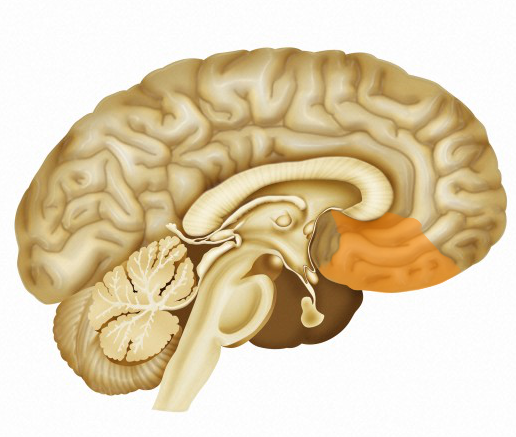
\includegraphics[width=.25\textwidth]{N0036253_mod.png}};
% \node[inner sep=0pt] (DLPFC) at (5,-6)
%     {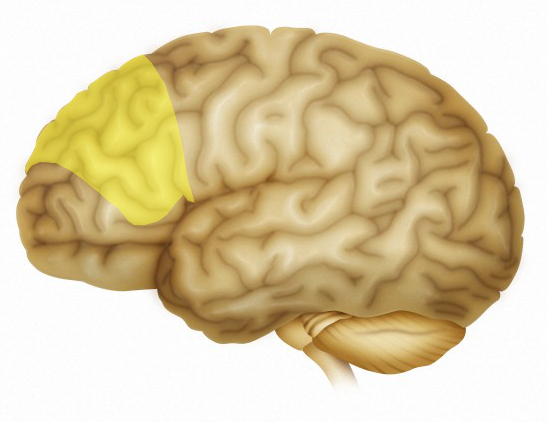
\includegraphics[width=.25\textwidth]{N0036254_mod.png}};



%\pgftext{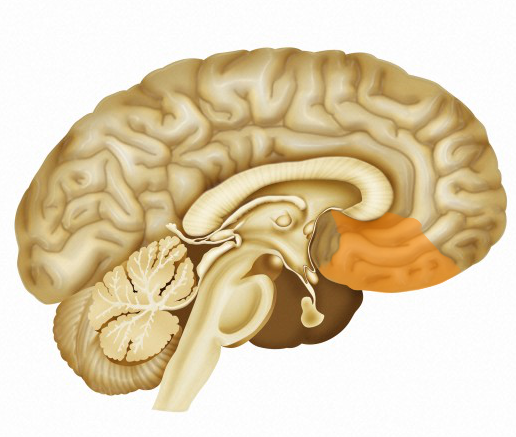
\includegraphics[width=150pt]{N0036253_mod.png}} at (5,5);
%\pgftext{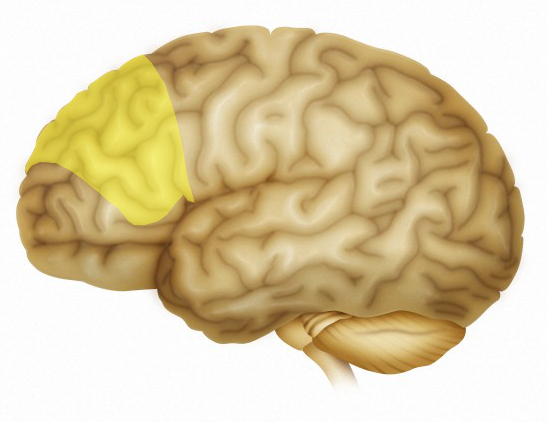
\includegraphics[width=150pt]{N0036254_mod.png}} at (7.85+7.85,-5.7-6.7);

\node (parenting_sit) at (13,6.7+3) 
  [draw
  ,circle
  ,minimum size=4cm
  ,align=center
  ,fill=nice_green
  ,line width=2.83464567pt
  ,draw=gray!60] 
  {\fontspec{Frutiger LT Std 55 Roman}Parenting \\ 
    \fontspec{Frutiger LT Std 55 Roman}Situation};

\node[draw
      ,circle
      ,minimum width=4cm
      ,fill=nice_green
      ,line width=2.83464567pt
      ,draw=gray!40
      ] (auto_mode) at (13,3)
    {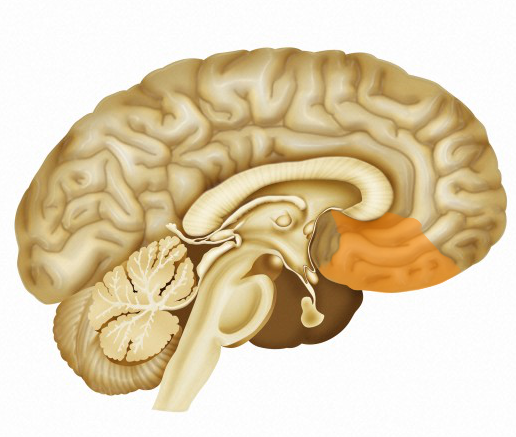
\includegraphics[width=.25\textwidth]{N0036253_mod.png}};
\node[draw=none] 
   (auto_mode_cover) at (13,1.5) {\fontspec{Frutiger LT Std 55 Roman}Automatic};

\node[draw
      ,circle
      ,minimum width=4cm
      ,fill=white
      ,line width=2.83464567pt
      ,draw=gray!40
      ] (manual_mode) at (7,3)
    {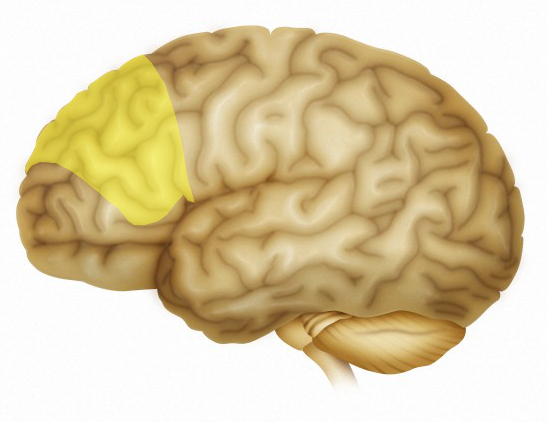
\includegraphics[width=.25\textwidth]{N0036254_mod.png}};
\node[draw=none] 
   (auto_mode_cover) at (7,1.5) {\fontspec{Frutiger LT Std 55 Roman}Manual};


\node[circle split
      ,draw,
      ,minimum width=4cm
      ,append after command={%
       \pgfextra{\draw (\tikzlastnode.center) -- (\tikzlastnode.south);
                 \draw[fill=nice_green
                      ,line width=2.83464567pt
                      ,draw=gray!40
                      ] (\tikzlastnode.west) arc (180:0:2cm) -- cycle;
                 \draw[fill=nice_green
                      ,line width=2.83464567pt
                      ,draw=gray!40
                      ] (\tikzlastnode.east) arc (0:180:2cm) -- cycle;
                 \draw[fill=nice_green
                      ,line width=2.83464567pt
                      ,draw=gray!40] (\tikzlastnode.center) -- (\tikzlastnode.west) arc (180:270:2cm) -- cycle;
                 \draw[fill=white
                      ,line width=2.83464567pt
                      ,draw=gray!40] (\tikzlastnode.center) -- (\tikzlastnode.east) arc (0:-90:2cm) -- cycle;
                } 
                }
        ]  at (13,-3.35) (parenting_beh)  {};
\node[yshift=2em, align=center] at (parenting_beh.center) 
  {\fontspec{Frutiger LT Std 55 Roman}Parenting \\ 
    \fontspec{Frutiger LT Std 55 Roman}Behavior};  
\node[xshift=-2.5em,yshift=-2.51em, align=center] at (parenting_beh.center) 
  {\fontspec{Frutiger LT Std 55 Roman}Optimal}; 
\node[xshift= 2.5em,yshift=-2em, align=center] at (parenting_beh.center) 
  {\fontspec{Frutiger LT Std 55 Roman}< \\
  \fontspec{Frutiger LT Std 55 Roman}Optimal};       

\node[circle split
      ,draw
      ,minimum width=4cm,
      ,append after command={%
       \pgfextra{\draw (\tikzlastnode.center) -- (\tikzlastnode.south);
                 \draw[fill=nice_green
                      ,line width=2.83464567pt
                      ,draw=gray!40
                      ] (\tikzlastnode.west) arc (180:0:2cm) -- cycle;
                 \draw[fill=nice_green
                      ,line width=2.83464567pt
                      ,draw=gray!40
                      ] (\tikzlastnode.east) arc (0:180:2cm) -- cycle;
                 \draw[fill=nice_green
                      ,line width=2.83464567pt
                      ,draw=gray!40] (\tikzlastnode.center) -- (\tikzlastnode.west) arc (180:270:2cm) -- cycle;
                 \draw[fill=white
                      ,line width=2.83464567pt
                      ,draw=gray!40] (\tikzlastnode.center) -- (\tikzlastnode.east) arc (0:-90:2cm) -- cycle;
                } 
                }
        ] at (13,-3.35-6.7) (child_wb)  {};
\node[yshift=2em, align=center] at (child_wb.center) 
  {\fontspec{Frutiger LT Std 55 Roman}Child \\ 
    \fontspec{Frutiger LT Std 55 Roman}Wellbeing};  
\node[xshift=-2.5em,yshift=-1.955em, align=center] at (child_wb.center) 
  {\textbf{\fontspec{Frutiger LT Std 55 Roman}\char"2265} \\
  \fontspec{Frutiger LT Std 55 Roman}Threshold}; 
\node[xshift= 2.5em,yshift=-2em, align=center] at (child_wb.center) 
  {\fontspec{Frutiger LT Std 55 Roman} < \\
  \fontspec{Frutiger LT Std 55 Roman}Threshold};   
% \node (parenting_beh) at (13,-3.35) 
%   [circle, draw, minimum size=22mm,align=center] 
%   {\fontspec{Frutiger LT Std 55 Roman}Parenting \\ 
%     \fontspec{Frutiger LT Std 55 Roman}Behaviors \\
%     \emph{\fontspec{Frutiger LT Std 55 Roman}Maltreative} \\
%     \emph{\fontspec{Frutiger LT Std 55 Roman}or Not}};

% \node (parenting_beh) at (13,-3.35) 
%   [circle, draw, minimum size=22mm,align=center] 
%   {\fontspec{Frutiger LT Std 55 Roman}Parenting \\ 
%     \fontspec{Frutiger LT Std 55 Roman}Behaviors};

% \node (child_wb) at (13,-3.35-6.7) 
%   [draw,circle, minimum size=22mm,align=center] 
%   {\fontspec{Frutiger LT Std 55 Roman}Child \\ 
%     \fontspec{Frutiger LT Std 55 Roman}Wellbeing};

\draw[->,line width=2.83464567pt]  
  (parenting_sit) to node [auto] {} (auto_mode);
  
\draw[->,line width=2.83464567pt]  
  (auto_mode) to node [auto] {} (parenting_beh);  
  
\draw[->,line width=2.83464567pt, align=center, draw=gray!40, bend right]  
  (auto_mode) to node [above=40pt, auto] 
    {\fontspec{Frutiger LT Std 55 Roman}Manual Mode \\
    \fontspec{Frutiger LT Std 55 Roman}Transition (Tx)} 
  (manual_mode);  

\draw[->,line width=2.83464567pt, bend right, draw=gray!40]  
  (manual_mode) to node [auto] {} (parenting_beh);  

\draw[->,line width=2.83464567pt]  
  (parenting_beh) to node [auto] {} (child_wb);

\node (wbar) at (8,1.25-6.7*2) [draw=none,fill=none] 
  {\fontspec{Frutiger LT Std 55 Roman} State Wellbeing Threshold};
\node (wbar_arrow_end) at (5,.9-6.7*2) [draw=none,fill=none] {};

\draw[->,bend left, line width=2.83464567pt]  (wbar) to node [auto] {} (wbar_arrow_end);


\end{tikzpicture}
\end{document}
